\section*{4.1 Vector spaces and subspaces}
  \subsection*{Theory}
 
    \subsubsection*{Vector Space}
    \begin{mydef}\label{vector space}
      A vector space is a nonempty set $ V $ of objects, called vectors, on which are fefined two operations, called addition and multiplication by scalars (real numbers), subject to the ten axioms listed below. The axioms must hold for all vectors $ \mathbf u, \mathbf v $ and  $ \mathbf W $ in $ V $ and for all scalars $ c $ and $ d $.
      \begin{enumerate}
        \item The sum of $ u $ and $ v $, denoted by $ \mathbf u + \mathbf v $, is in $ V $
        \item $ \mathbf u + \mathbf v = \mathbf v + \mathbf u $
        \item $ (\mathbf u + \mathbf v) + \mathbf w = \mathbf u + (\mathbf v + \mathbf w)  $
        \item There is a zero vector $ \vec{0} $ in $ V $ such that $ \mathbf u + \mathbf 0 = u $
        \item For each $ \mathbf u $ in $ V $, there is a vector $ - \mathbf u $ in $ V $ such that $ \mathbf u + (-\mathbf u) = 0 $
        \item The scalar multiple of $ u $ by $ c $ denoted by $ c \mathbf u $ is in $ V $
        \item $ c (\mathbf{u + v}) = c \mathbf u + c \mathbf v $
        \item $ (c+d)\mathbf u = c \mathbf u + d \mathbf u $
        \item $ c(d \mathbf u) = (cd) \mathbf u $
        \item $ 1 \mathbf u  = \mathbf u $
      \end{enumerate}

    \end{mydef}

    \begin{mydef}\label{subspace}
      A subspace of a vector space V is a subset H of V that has three properties:
      \begin{itemize}
        \item The zero vector of V is in H
        \item $H$ is closed under vector addition. That is, for each $  \mathbf  u $ and $ \mathbf  v$ in $H$, the sum $ \mathbf  u$ $C$ $ \mathbf  v$
        is in $H$
        \item $H$ is closed under multiplication by scalars. That is, for each $ \mathbf  u$ in $H$ and each
        scalar $c$, the vector $c \mathbf  u$ is in $H$        
      \end{itemize}
    \end{mydef}

    \begin{theorem} \label{Theorem 1}
      If $ \vec{v_1}, \dots, \vec{v_n} ∈ V$ then $ span\{\vec{v_1}, \dots, \vec{v_n}\} $ is a subspace of $ V $ 
    \end{theorem}

  \subsection*{Exercises}
    \subsubsection*{12}

    Let $ W $ be the set of all vectors of the form $   \begin{pmatrix}
         s + 3t   \\ 
         s - t \\ 
         2s - t \\
         4t
      \end{pmatrix} $. 
    Show that $ W $ is a subspace of $ \mathbb R^{4} $. \newline \newline 

    \bf{Solution} \newline \newline 
    We can split $ W $ up into a sum of other vectors. 
    $$
        \begin{pmatrix}
          s + 3t   \\ 
          s - t \\ 
          2s - t \\
          4t
        \end{pmatrix} = 
     s   \begin{pmatrix}
          1  \\ 
          1  \\ 
          2  \\
          0  
       \end{pmatrix} + 
    t   \begin{pmatrix}
         3  \\ 
         -1  \\ 
         -1  \\
         4  
      \end{pmatrix}
    $$
    \[
    W = span \left\{
      \begin{pmatrix}
        1  \\ 
        1  \\ 
        2  \\
        0  
     \end{pmatrix} , 
     \begin{pmatrix}
       3  \\ 
       -1  \\ 
       -1  \\
       4  
    \end{pmatrix}
    \right\}_{}^{} 
    \]
    \cref{Theorem 1} says $ W $ is a subspace of $ \mathbb R^{4} $
    
    
    
    \subsubsection*{40}
    Let $ H $ and  $ K $ be subspaces of a vector space $ V $. The intersection of $ H $ and $ K $, written $ H \bigcap K $ is a subspace of $ V $. Give an example in $ \mathbb R^{2}  $ to show that the union of two subspaces is not, in general, a subspace 
    \begin{figure}[h!]
      \centering
      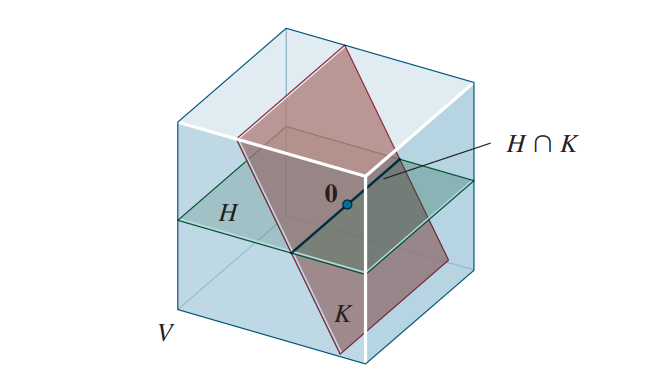
\includegraphics[scale = .7]{Bilder/HK_intersect.png}
      \caption{}
      \label{fig:figure1}
    \end{figure}
    \newline \newline 

    \bf{Solution} \newline \newline 
    The intersection of the two planes creates a line going across the x-axis which we already know is a subspace of both $ \mathbb R^{3} $ and $ \mathbb R^{2} $. Same goes for all straight lines going trough origin. \newline 
    The union of two subspaces, (lets use the x and y-axis) will often create vectors outside the subspace, thus not being closed by addition. If we take a vector from the x-axis and a vector from the y-axis and add them together, they will create a vector outside both axis. 

    \bf{Solution} \newline \newline 
    \subsubsection*{44}
    Determine if $ \mathbf y $ is in the subspace of $ \mathbb R^{4} $ spanned by the collumns of $ A $, where
    \[
    \mathbf y = 
    \begin{pmatrix}
       -4  \\ 
       -8  \\ 
       6  \\
       -5  
    \end{pmatrix}, \quad
    A = \begin{pmatrix}
      3 & -5 & -9 \\ 
      8 & 7 & -6 \\ 
      -5 & -8 & 3 \\ 
      2 & -2 & -9
    \end{pmatrix}
    \]
    \newline \newline 
    \bf{Solution} \newline \newline 
    We can divide $ A $ into three vectors where each one is a column in $ A $. If these three vectors can form a linear combination which can create $ \mathbf y $ (in other words, $ \mathbf y $ is in the span of these vectors), then $ \mathbf y $ will be in the subspace of $ \mathbb R^{4}$ spanned by the columns of $ A $. To test this we append the vector $ \mathbf y $ to the end of $ A $ and then reduce it to row echelon form. 
    \begin{figure}[h!]
      \centering
      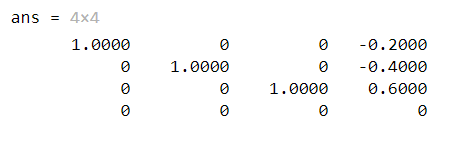
\includegraphics[scale = .7]{Bilder/Exercise_44_matlab.png}
      \caption{Results using matlab}
      \label{fig:figure1}
    \end{figure}
    As seen above the equation has a solution which means $ \mathbf  y $ is in the subspace of $ \mathbb R^{4}$ spanned by the columns of $ A $.

\section*{4.2 Null Spaces, Column Spaces, Row Spaces, and Linear Transformations}
  \subsection*{Theory}
    \subsubsection*{The Null Space of a Matrix}

    

    \begin{mydef}\label{def: null space}
      The \bf{null space} of an $ m × n $ matrix $ A $, written as Nul $ A $, is the set of all solutions of the homogenous equation $ A \mathbf x = \mathbf 0 $. In set notation, 
      \[
      \operatorname{Nul} A = \left\{\mathbf x: \mathbf x \text{ is in } \mathbb R^{n}  \text{ and } A \mathbf x = \mathbf 0 \right\}_{}^{}
      \]
      
      
      
    \end{mydef}    

    \begin{figure}[h!]
      \centering
      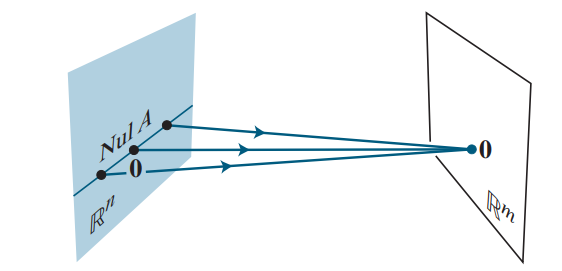
\includegraphics[scale = .7]{Bilder/nullspace_figure.png}
      \caption{Visualization of the subspace (in this case a line) formed by the null space of $ A $}
      \label{fig:figure1}
    \end{figure}

    \begin{theorem} \label{theorem: null space}
      The null space of an $ m × n  $ matrix $ A $ is a subspace of $ \mathbb R^{n} $. Equivalently, the set of all solutions to a system $ A \mathbf  x = \mathbf  0 $ of $ m  $ homogeneous linear equations in $ n $ unknowns is a subspace of $ \mathbb R^{n} $. 
    \end{theorem}

    \subsubsection*{The Column Space of a Matrix}
      \begin{mydef}\label{def: column space}
        The Column space of an $ m × n $ matrix $ A $, written as Col $ A $, is the set of all linear combinations of the columns of $ A $. If $ A = \left[\mathbf a_1 \dots \mathbf a_n\right]_{}^{} $, then 
        \[
        Col \ A = Span = \left\{\mathbf a_1 \dots \mathbf a_n\right\}_{}^{} 
        \]
      \end{mydef}

      \begin{theorem}\label{theorem: column space}
        The column space of an $ m × n $ matrix $ A $ is a subspace of $ \mathbb R^{n} $. 
      \end{theorem}

    \subsection*{Exercises}
      \subsubsection*{4}
        Find the explicit definition of Nul $ A $ by listing vectors that span the null space. 
        \[
        A = \begin{bmatrix}
          1 & -6 & 4 & 0\\ 
          0 & 0 & 2 & 0
        \end{bmatrix}
        \]

        \bf{Solution} \newline \newline 
        We start by reducing it to echelon form multiplying by $ \mathbf x $ and set as equal to the zero vector. 
        \[
        A \mathbf x = \mathbf 0
        \]
        \[
        rref(A) = \begin{bmatrix}
          1 & -6 & 0 & 0\\ 
          0 & 0 & 1 & 0
        \end{bmatrix}
        \]
        \[
          \begin{bmatrix}
            1 & -6 & 4 & 0\\ 
            0 & 0 & 2 & 0
          \end{bmatrix} 
          \mathbf x = 
          \begin{pmatrix}
             0  \\ 
             0 
          \end{pmatrix}
        \]
        \[
        \mathbf x = \begin{pmatrix}
           0  \\ 
           0  \\ 
           0  \\
           0  
        \end{pmatrix}
        \]
        \[
        Nul \ A = span \left\{\begin{pmatrix}
          0  \\ 
          0  \\ 
          0  \\
          0  
       \end{pmatrix}\right\}_{}^{} 
        \]

      \subsubsection*{52}
      Let $ H = Span\{\mathbf v_1, \mathbf v_2\} $ and $ K = Span\{\mathbf v_3, \mathbf v_4\}$, where 
      \[
      \mathbf v_1 = \begin{pmatrix}
         5  \\ 
         3  \\ 
         8 
      \end{pmatrix}, 
      \mathbf v_2 = \begin{pmatrix}
         1  \\ 
         3  \\ 
         4 
      \end{pmatrix}, 
      \mathbf v_3 = \begin{pmatrix}
         2  \\ 
         -1  \\ 
         5 
      \end{pmatrix}, 
      \mathbf v_4 = \begin{pmatrix}
         0  \\ 
         -12  \\ 
         -28 
      \end{pmatrix} 
      \]
      Then $ H $ and $ K $ are subspaces of $ \mathbb R^{3} $. In fact, $ H $ and $ K $ are planes in $ \mathbb R^{3} $ through origin, and they intersect in a line through $ \mathbf 0 $. Find a nonzero vector $ \mathbf w $ that generates that line. [Hint: $ \mathbf w $ can be written as $ c_1 \mathbf v_1 + c_2 \mathbf v_2 $ and also as $ c_3 \mathbf v_3 + c_4 \mathbf v_4 $. To build $ \mathbf w $, solve the equation $ c_1 \mathbf v_1 + c_2 \mathbf v_2  = c_3 \mathbf v_3 + c_4 \mathbf v_4  $ for the unknown $ c_j $'s] \newline \newline
      \bf{Solution} \newline \newline 
      
\section*{4.3 Linearly Independent Sets; Bases}
  \begin{theorem}
    And indexed set $ \left\{ \mathbf{v}_1,\mathbf{v}_2,\cdots,\mathbf{v}_p \right\}  $ of two or more vectors, with $ \mathbf{v}_1 \neq  \mathbf{0} $, is linearly dependent if and only if some $ \mathbf{v}_j $
    with j > 1 is a linear combination of the preceding vectors $ \mathbf{v}_1 \cdots \mathbf{v}_{j - 1} $.  \end{theorem}
  
  \begin{mydef}
    Let H be a subspace of a vector space $ V $. A set of vectors $ \mathcal{B} $ in $ V $ is a basis for $ H $ if 
    \begin{itemize}
    \item  $ \mathcal{B} $ is a linearly independent set, and 
    \item the subspace spanned by $ B_c $ coincides with $ H $; that is, 
    \end{itemize}
    \[
    H = Span \ \mathcal{B}
    \]
  \end{mydef}

  \subsection*{Exercises}
    \subsubsection*{12}
      Find a basis for the set of vectors in $ \mathbb{R}^{2}  $ on the line $ y = 5x  $. \newline \newline 
      \bf{Solution} \newline \newline 

      \[
      x \begin{pmatrix} 1 \\ 0 \\\end{pmatrix} + 
      x \begin{pmatrix} 0 \\ 5 \\\end{pmatrix} = \begin{pmatrix} x \\ 5x \\\end{pmatrix}
      \]
    
    \subsubsection*{13}
      Find bases for $ \operatorname{Nul}A $, $ \operatorname{Col}A $ and $ \operatorname{Row}A $. 
      \[
      A = 
      \begin{bmatrix*}[r]
       -2 & 4 & -2 & -4 \\
       2 & -6 & -3 & 1 \\
       -3 & 8 & 2 & -3 
      \end{bmatrix*}, 
      B = 
      \begin{bmatrix}
       1 & 0 & 6 & 5 \\
       0 & 2 & 5 & 3 \\
       0 & 0 & 0 & 0
      \end{bmatrix}
      \]
      
      \bf{Solution} \newline \newline
      Get matrix $ A $ in echelon form and you will se the rows of $ A $ and $ B $ are equivalent. This means the space spanned by the vectors making the rows of $ A $ and $ B $ (Row $ A $) is equal. We find Col $ A $ by looking at the linearly independent columns of $ B $. We find $ \operatorname{Nul}A $ by solving the equation $ A \mathbf{x} = \mathbf 0 $. 
      \[
      \operatorname{Nul}A = \left\{ 
        \begin{pmatrix*}[r]
         -6 \\
         -\frac{5}{2} \\
         1 \\
         0 \\
        \end{pmatrix*}, 
        \begin{pmatrix*}[r]
         -5 \\
         -\frac{3}{2} \\
         0 \\
         1 \\
        \end{pmatrix*}
       \right\}, \quad
       \operatorname{Col}A = \left\{ 
        \begin{pmatrix*}[r]
         -2 \\
         2 \\
         -3 \\
        \end{pmatrix*}, 
        \begin{pmatrix*}[r]
         4 \\
         -6 \\
         8 \\
        \end{pmatrix*}
        \right\} , \quad
        \operatorname{Row}A = \left\{
          \begin{pmatrix*}[r]
           1 & 0 & 6 & 5 \\
          \end{pmatrix*}, 
          \begin{pmatrix*}[r]
           0 & 2 & 5 & 3 \\
          \end{pmatrix*}
        \right\}_{}^{} 
      \]

    \subsubsection*{36}  
      In the vector space of all real-valued functions, find a basis for the subspace spanned by $ \{ \sin t, \sin 2t, \sin t, \cos t \}$. 

\section*{4.4 Coordinate Systems}
  \subsection*{Theory}
    We can use a basis in a given dimension as a tool to create a new coordinate system. 
    
    \begin{theorem}[The Uniqe Representation Theorem]\label{The Uniqe Representation Theorem}
      Let $ \mathcal{B} = \{ \mathbf{b}_1,\mathbf{b}_2,\cdots,\mathbf{b}_n \} $ be a basis for a vector space $ V $. Then for each $ \mathbf{x} $ in $ V $, there exist a unique set of scalars $ c_1,c_2,\cdots,c_n $ such that
      \[
      \mathbf{x} = c_1 \mathbf{b}_1+c_2 \mathbf{b}_2+\cdots+c_n \mathbf{b}_n
      \]
    \end{theorem}
  \subsection*{Exercises} 
    \subsubsection*{3}
    Find the vector $ \mathbf{c} $ determined by the given coordinate vector $ \left[ \mathbf{x} \right] _{\mathcal{B}} $, and the given basis $ \mathcal{B} $
    \[ 
      \mathcal{B} = \left\{ 
        \begin{pmatrix*}[r]
         1 \\
         -8 \\
          6
        \end{pmatrix*}, 
        \begin{pmatrix*}[r]
         2 \\
         -5 \\
         7
        \end{pmatrix*}, 
        \begin{pmatrix*}[r]
         3 \\
         9 \\
         -4 \\
        \end{pmatrix*}
        \right\}
        \left[ \mathbf{x} \right] _{\mathcal{B}} = \begin{pmatrix*}[r]
         2 \\
         -3 \\
         0 \\
        \end{pmatrix*}
    \]

\bf Solution \newline \newline 

We put the vectors forming the basis $ \mathcal{B} $ in a matrix and reduce it to echelon form
\[
\begin{bmatrix*}[r]
 1 & 2 & 3 \\
 -8 & -5 & 9 \\
 6 & 7 & -4 \\
\end{bmatrix*} → \left(\begin{array}{rrrr}1&0&0&\frac{73}{22} \\ 0&1&0&\frac{-5}{2}\\0&0&1&\frac{27}{22}\\\end{array}\right)
\]



    

        
